\documentclass{article}

\usepackage{booktabs}
\usepackage{tabularx}
\usepackage{enumitem}
\usepackage{tikz}
\usepackage[normalem]{ulem} % for strikethrough
\usetikzlibrary{positioning, shapes, arrows.meta}

\title{Development Plan\\\progname}

\author{\authname}

\date{}

\input{../Comments}
%% Common Parts

\newcommand{\progname}{Industrial Plant Designer} % PUT YOUR PROGRAM NAME HERE
\newcommand{\authname}{Team 18, Chemware Engineering
\\ Kishor Pandya
\\ Dhrumil Pandya
\\ Madhu Sivapragasam
\\ Rasik Pokharel} % AUTHOR NAMES                  

\usepackage{hyperref}
    \hypersetup{colorlinks=true, linkcolor=blue, citecolor=blue, filecolor=blue,
                urlcolor=blue, unicode=false}
    \urlstyle{same}
                                


\begin{document}

\maketitle

\begin{table}[hp]
\caption{Revision History} \label{TblRevisionHistory}
\begin{tabularx}{\textwidth}{llX}
\toprule
\textbf{Date} & \textbf{Developer(s)} & \textbf{Change}\\
\midrule
September 17th & Madhu Sivapragasam & Add intro and expected technology\\
September 18th & Kishor Pandya & Add team meeting plan, communication plan, and member roles\\
September 21st & Madhu Sivapragasam & Added appendix answers\\
September 22nd & Dhrumil Pandya & Added project decomposition and scheduling\\
September 23rd & Dhrumil Pandya & Added workflow plan\\
September 23rd & Dhrumil Pandya & Added coding standard, POC Demo Plan and reflection \\
September 23rd & Kishor Pandya & Added answer to appendix\\
September 23rd & Rasik Pokharel & Added copyright, ip to protect and confidential information sections \\ 
November 12th & Dhrumil Pandya & Modified Scheduling Approach\\
April 3rd & Madhu Sivapragasam & Updates for revision 1\\
\bottomrule
\end{tabularx}
\end{table}

\newpage{}

This document is intended to cover the overall development plan for the User Interface and Model Version Management for Models of Industrial Plants project. The document will cover all necessary information for the development process of the project including team information, development information, information related to IP as well as other related subjects. 

\section{Confidential Information?}

This project may involve certain confidential information that must be handled with care to ensure the privacy and security of data. The following outlines the types of confidential information and the protective measures to be implemented:

\subsection*{Types of Confidential Information}
\begin{itemize}
    \item \textbf{Proprietary Plant Data:} Detailed operational data of the chemical plant, including process parameters, production rates, and chemical formulations, which are proprietary to the plant and must be safeguarded.
    \item \textbf{Simulation Models:} Existing Python scripts and simulation models provided by the plant or other stakeholders, containing sensitive algorithms and methods for plant operation.
    \item \textbf{User Data:} Information entered into the system by users, such as user configurations, preferences, and any personal data associated with user accounts.
\end{itemize}

\subsection*{Data Protection Measures}
\begin{itemize}
    \item \textbf{Access Control:} Implementing strict access control measures to ensure that only authorized individuals can access confidential data. This includes secure login systems for accessing the software and the database.
    \item \textbf{Secure Data Storage:} Using secure database systems and servers with regular security updates to store confidential information safely.
    \item \textbf{Non-Disclosure Agreements (NDAs):} Ensuring all team members and stakeholders involved in the project sign NDAs and other legal documentation to legally protect the confidentiality of sensitive information. This process will be facilitated by Dr. Smith and Dr. Mahalec as directed by appropriate McMaster, policies and guidelines.

\end{itemize}

\section{IP to Protect}
This project involves the development and use of intellectual property (IP) that must be protected to maintain the rights and interests of all stakeholders involved. The following outlines the types of IP and the strategies for their protection:

\subsection*{Types of Intellectual Property}
\begin{itemize}
    \item \textbf{Software Code:} The newly developed front-end GUI software and the database system, including any custom algorithms, user interface designs, and data processing techniques created as part of this project.
    \item \textbf{Plant Simulation Models:} Existing Python scripts and models provided for this project, which may include proprietary algorithms and methods for modeling the chemical plant.
    \item \textbf{Database Structures:} The schema and organization of the database that models the plant's operations, which may include innovative data structures and relationships designed to optimize plant performance.
    \item \textbf{Project Documentation:} Detailed documentation, including design specifications, user manuals, and technical reports, which provide valuable insights into the design and operation of the software.
\end{itemize}

\subsection*{Protection Strategies}
\begin{itemize}

    \item \textbf{Code Repositories:} Using only GitHub and GitLab to prevent unauthorized access to the source code and related project files. Only sharing to appropriate stakeholders and keeping repos private.
    \item \textbf{Documentation Control:} Marking documentation containing IP or confidential data as confidential and controlling its distribution to prevent unauthorized sharing of information. 

\end{itemize}


\section{Copyright License}
The intellectual property (IP) developed during this project, including the software code, graphical user interface (GUI), database structures, and documentation, is protected under copyright law. 
We will be using a licensing model that restricts the reuse of the developed software for this project. As a part of the capstone agreement, Dr. Mahalec has agreed to purchase the IP of this project upon successful delivery of project requirements.
We will be using a Proprietary Software licence for this project. This license is included in the root of our project repo and outlines that unauthorized sharing or use of this software is prohibited. 


\section{Team Meeting Plan}

Team 18 is planning on meeting three times per week. 
Two of the meetings will include our supervisor, and one meeting will be amoung just the developers. 
Apart from these scheduled meetings, team members can schedule impromtu meetings with eachother to work on the project and get help.\\ \\
The current scheduled meetings are as follows:
\begin{itemize}
  \item Monday 1:00 PM to 1:30 PM, this meeting will be held virtually through MS Teams and will include our supervisor.
  \item Monday 6:00 PM to 7:00 PM, this meeting will be held virtually through Discord and will only include the team members.
  \item Thursday 11:45 AM to 1:15 PM, this meeting will be held in-person and will include the supervisor.
\end{itemize}

Each of the three meetings has a specific purpose. The first meeting on Monday is a short one where the team members will update the supervisor on the work done in the previous week and the plan for this current week. \\

The next meeting on Monday is setup to be a scrum meeting amoung the developers. In this meeting the developers are expected to create new issues based on the required work and assign the work amoung themselves. This meeting will also include developers informing other developers of roadblocks that they are running into. \\

The last meeting of the week which is scheduled for Thursday will include the supervisor. This will be a longer meeting in comparion, here the team along with our supervisor will plan for the next stages of the project. This meeting will also include any changes that will be made to the current plan depending upon how the project is coming along. The chair for the meetings will be Kishor Pandya.
\section{Team Communication Plan}

The team members have a Discord channel setup for all communication among themselves.\\
The team also has a MS Teams channel setup with the supervisor for information to be relaied between the team and supervisor.\\
We have also setup a Github projects page to keep track of tasks and issues. New tasks will be added each week as the project is built. The tasks will make use of Github issues by creating a ticket for each task.\\

\section{Team Member Roles}

\subsection{Team Leader}
The team leader is Madhu Sivapragasam.\\
\textbf{Responsibilities}: To make sure that all members are equally contributing to the project. The team leader must also communicate with the course instructor.
\textbf{Role change}: \textcolor{blue}{Kishor Pandya will also take the role of leader if Madhu is otherwise busy or not available}

\subsection{Meeting chair}
The meeting chair is Kishor Pandya.\\
\textbf{Responsibilities}: To prepare and manage meetings but setting up meeting goals. The meeting chair must also resolve any disputes that occur during the meetings and must maintain the a professional standard during the meetings.
\textbf{Role change}: \textcolor{blue}{If Kishor is not available, the other 3 group members will rotate the meeting chair responsibilities}

\subsection{Notetaker}
The notetaker is Dhrumil Pandya and Rasik Pokharel.\\
\textbf{Responsibilities}: To take meeting minutes for each meeting, summarize them so that everyone can refer to them later on.
\textbf{Role change}: \textcolor{blue}{In case both Dhrumil and Rasik are not available than Kishor will take over notetaker duties.}

\subsection{Reviewer}
There is no fixed reviewer for the project. For each PR, the author must assign one other team member (not themselves) as the primary reviewer, and at least one approval is required before merging.\\
\textbf{Responsibilities}: To review the work done by their fellow teammate, catch mistakes and ask the member working on that to resolve the issues found.

\section{Workflow Plan}

For this Capstone project, we want to use a workflow that keeps things organized but isn't overly complicated. Since we're all familiar with GitHub projects and repository, we're using them to manage our code and collaborate. 
Here is the detailed breakdown:


\subsubsection{Git Usage}

We've set up a private GitHub repository (requested by our sponsor to make it private) for our project to keep everything including code and documentation in one place.

\begin{itemize}
    \item \textbf{Main Branch (\texttt{main})}: This is our stable branch where the latest working code resides. We try not to commit directly to \texttt{main} to avoid introducing any issues.

    \item \textbf{Feature Branches}: Whenever someone starts working on a new feature or bug fix, they create a new branch off of \texttt{main}. We name these branches after the GitHub issue they're addressing, like \texttt{feature/login-backend-work} or \texttt{doc/workflow-plan}. This makes it easy to see what each branch is about.
\end{itemize}

After finishing work on a feature, we open a \textbf{Pull Request (PR)} to merge the changes back into \texttt{main}. We make sure to link the PR to its corresponding issue for clarity and assign another team member as reviewer.

\subsubsection{Pull Requests and Code Review}

For PRs, we require the PR author to select another team member as reviewer before requesting approval. At least one team member must review and approve the changes before merging. This helps us catch any potential problems early and ensures that everyone is aware of changes happening in the codebase. During the review, we focus on:

\begin{itemize}
    \item \textbf{Functionality}: Does the code do what it's supposed to?

    \item \textbf{Code Quality}: Is the code clean and maintainable? (CI should also be able to catch this)
\end{itemize}

Once the PR is approved, we merge it into \texttt{main} and delete the feature branch to keep things uncluttered.

\subsubsection{Issue Management}

To keep track of tasks and bugs, we're using \textbf{GitHub Issues}. Here's the breakdown:

\begin{itemize}
    \item \textbf{Creating Issues}: For every task, whether it's a new feature, an improvement, or a bug fix, we create a GitHub Issue. We include a clear title and a detailed description.

    \item \textbf{Issue Templates}: For the issue template we have created a generic template that can be used for the Github Issues. The `markdown` file below

    \begin{verbatim}
        **Description**
        A clear and concise description of the bug/feature

        **Expected Behavior**
        Describe what you expect to happen through this bug fix/feature

        **Related screenshots**
        If applicable, add screenshots or logs for the feature/issue
    \end{verbatim}

    \item \textbf{Labels and Classification}: We use labels to categorize issues, which helps in filtering for metrics:

    \begin{itemize}
        \item \textbf{Type}: \texttt{bug}, \texttt{feature}, \texttt{chore}, \texttt{documentation}

        \item \textbf{Area}: \texttt{frontend}, \texttt{backend}, \texttt{database/modelling}, \texttt{infra}
    \end{itemize}

    \item \textbf{Assignment}: We assign issues to team members based on their areas of expertise/interests. The issue will be assigned when they are created. If the issue is created by the TA/sponsor/prof we will triage it based on the expertise of the team member.
\end{itemize}

\subsubsection{Project Management}

We're using the \textbf{GitHub Projects} to organize our workflow. Our project board is set up with columns:

\begin{itemize}
    \item \textbf{To Do}: Issues that are ready to be worked on.

    \item \textbf{In Progress}: Issues that someone is currently working on.

    \item \textbf{Code review}: Completed work that's awaiting review.

    \item \textbf{Done}: Tasks that have been completed and merged.
\end{itemize}

As we work on issues, we move them across the board to reflect their status.

\subsubsection{Continuous Integration/Continuous Deployment (CI/CD)}

To maintain code quality and catch issues early, we will eventually set up Continuous Integration using \textbf{GitHub Actions}:

\begin{itemize}
    \item \textbf{Automated Testing}: Whenever we push code to \texttt{main} or open a PR, our test suite runs automatically when we set it up. As mentioned in the technology section below we will use \textbf{Jest} for unit tests, and as we build out our application.

    \item \textbf{Code Quality Checks}: We will have \textbf{ESLint} and \textbf{Prettier} configured to enforce consistent and clean coding styles. These tools run automatically during the CI process, it will flag if the linting issue needs to be resolved. 
\end{itemize}

At the initial stage, we're focusing on local development and testing, so we're not deploying to a live server yet. However, we're planning to implement Continuous Deployment in the future. Once we reach that point, our CI/CD pipeline will also handle deploying our application to the server when it passes all the CI steps.

\section{Project Decomposition and Scheduling}

For our capstone project, we will use \textbf{GitHub Projects} to organize and manage our tasks. This will help us visualize our workflow using Kanban board, allowing us to track progress from "To Do" to "In Progress", "Code Review" and to "Done." Additionally, we’ll use Outlook to schedule team meetings and set reminders for key milestones and deadlines. We also have Microsoft Teams chat setup with our supervisor and scheduled meeting with him for Mondays and Thursdays. As described in Team Meeting Plan. Additionally, we are using Discord for quick communication among team members. \href{https://github.com/users/MadhuranS/projects/1}{Link to GitHub Project (It is private on supervisor's demand)} and \href{https://github.com/MadhuranS/capstone}{Link to GitHub Repository (It is also private)}

\subsection{Scheduling Approach}
We plan to adopt an iterative (agile) approach, breaking down the project into four main phases from September to April. Each phase will focus on specific milestones, allowing us to tackle the project step-by-step while gathering feedback and making necessary adjustments along the way from Dr. Smith, TA, Supervisor and his team. This method makes this process flexible and allows us to address any challenges quickly. 

\subsubsection{Phases of this project}

\begin{itemize}
    \item \textbf{Phase 1: September to October}: During this initial phase, we will focus on team formation, project selection, and creating a comprehensive development plan. We will also begin learning the necessary technologies, such as React.js and React Flow, to build the GUI. Initial implementations, such as the basic drag-and-drop features, will be developed as they are foundation of the project

    \item \textbf{Phase 2: October to November}: In the second phase, we will focus towards designing and implementing the database. We will finalize the database schema for network topology and set up the SQL database. At the same time, we will start integrating the database with the API endpoints, setting up communication from database with backend. Initial testing and the Proof of Concept Demonstration will also take place during this phase.

    \item \textbf{Phase 3: December to February}: The third phase we will concentrate on completing the GUI functionality and fully integrating the Python model given by the supervisor's team with our system. We will also start the integration between the backend and frontend; so essentially the data on client side will be read from the database. We will develop backend APIs, link model results to the frontend, and do e2e testing. Additionally, we will work on the Design Document Revision 0.

    \item \textbf{Phase 4: March to April}: In the final phase, we will focus on final testing, preparing the V\&V Report, and compiling all necessary documentation. This phase will also include the Final Demonstration and the EXPO Demonstration. Final Documentation will be completed.
\end{itemize}

\subsubsection{Task Decomposition}
\begin{enumerate}
    \item \textbf{GUI Development}
    \begin{enumerate}[label=\alph*)]
        \item Complete a tutorial on React Flow and explore other libraries to create nodes and edges.
        \item Implement the drag-and-drop functionality for plant components, allowing users to place nodes on the canvas.
        \item Develop the feature to connect nodes with arcs, enabling users to create the plant network.
        \item Conduct tests on the drag-and-drop and connection features.
    \end{enumerate}

    \item \textbf{Database Design}
    \begin{enumerate}[label=\alph*)]
        \item Design the schema for storing network topology, including nodes and arcs.
        \item Set up the SQL database to store user configurations and model data.
        \item Integrate the database with the GUI, facilitating data flow between the frontend and backend.
        \item Test the database interactions with the UI to verify data integrity and functionality.
    \end{enumerate}

    \item \textbf{Integration with Python Model}
    \begin{enumerate}[label=\alph*)]
        \item Understand the existing Python plant model provided by Prof. Mahalec and brainstorm how to integrate it into the project.
        \item Develop backend APIs to facilitate communication between the GUI and the Python model.
        \item Link the model results to the frontend interface, allowing users to view simulation outputs.
        \item Test the integration to ensure accurate data flow and correct model outputs.
    \end{enumerate}

    \item \textbf{Testing}
    \begin{enumerate}[label=\alph*)]
        \item Write unit tests for GUI components to verify their functionality.
        \item Develop unit tests for database connections.
        \item Create integration tests to validate the interaction between different system components.
        \item Conduct end-to-end testing of the entire workflow.
    \end{enumerate}
\end{enumerate}

\subsection{Assignment and Time Allocation}

Tasks will be assigned based on each team member’s strengths and interests. During our weekly meetings, we will discuss task assignments to make sure that everyone is working on areas where they can contribute most effectively. Team members will also participate in code reviews, which will help fill any knowledge gaps that might arise for developers not actively working on that feature
\newline
\\
Considering that each team member can dedicate around 10 hours per week in addition to the allocated capstone lecture and tutorial time to the project, our total team effort is approximately 40 hours per week. We will distribute and break down tasks accordingly to ensure weekly deliverables are met

\subsubsection{Documentation Process and Deliverable Breakdown}

\begin{enumerate}
    \item September: Team formation, project selection, and initial development plan.
    \item October: Completion of the Requirements Document and Hazard Analysis.
    \item November: Proof of Concept Demonstration.
    \item January: Design Document Revision 0.
    \item March: V\&V Report and Final Demonstration.
    \item April: Final Documentation and EXPO Demonstration.
\end{enumerate}

\textbf{Documentation and phases}
\newline
\newline
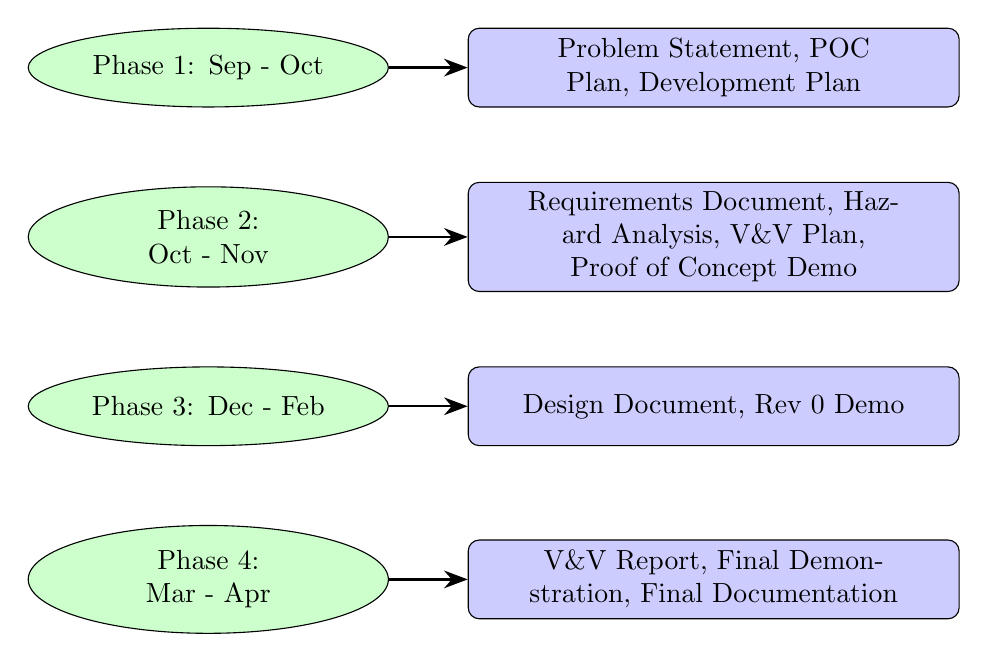
\begin{tikzpicture}[
    milestone/.style={rectangle, draw, rounded corners, fill=blue!20, text width=6cm, align=center, minimum height=1cm},
    phase/.style={ellipse, draw, fill=green!20, text width=3cm, align=center, minimum height=1cm},
    arrow/.style={-{Stealth[length=3mm]}, thick}
]

% Phases
\node (phase1) [phase] {Phase 1: Sep - Oct};
\node (phase2) [phase, below=of phase1] {Phase 2: Oct - Nov};
\node (phase3) [phase, below=of phase2] {Phase 3: Dec - Feb};
\node (phase4) [phase, below=of phase3] {Phase 4: Mar - Apr};

% Milestones
\node (ms1) [milestone, right=of phase1] {Problem Statement, POC Plan, Development Plan};
\node (ms2) [milestone, right=of phase2] {Requirements Document, Hazard Analysis, V\&V Plan, Proof of Concept Demo};
\node (ms3) [milestone, right=of phase3] {Design Document, Rev 0 Demo};
\node (ms4) [milestone, right=of phase4] {V\&V Report, Final Demonstration, Final Documentation};

% Arrows
\draw [arrow] (phase1) -- (ms1);
\draw [arrow] (phase2) -- (ms2);
\draw [arrow] (phase3) -- (ms3);
\draw [arrow] (phase4) -- (ms4);

\end{tikzpicture}

\section{Proof of Concept Demonstration Plan}

\subsubsection{Identified Risks and Mitigation Strategies}

\begin{enumerate}
    \item \textbf{User Interface (UI) Usability}: One of the main risks is making sure that our user interface is both intuitive and functional. Since we’re building a drag-and-drop system for designing power plants, there’s a possibility that users might find it difficult to add or connect components smoothly. To mitigate this, our POC will show a basic version of the UI using React and the React-flow library. We will demo key functionalities such as dragging components onto the canvas, connecting them, and assigning basic parameters (defined by supervisor). Successfully presenting these features will confirm that our chosen tools and design approach can support the necessary UI requirements.
    \item \textbf{Handling JSON Data with Dual Databases}: Another significant challenge is managing the JSON data generated by the React-flow diagrams alongside our dual-database setup (the dual db setup is requirement by the supervisor). The user database, which stores the drawn plant maps, may require a NoSQL approach due to the JSON structures, while the system database, containing all icons and system information, will remain SQL-based for its structured data. This dual-db system introduces complexity in ensuring data consistency. During our POC, we will demo how JSON output from React-flow is parsed and stored in the user database while maintaining references to the system SQL database. This involves creating a simple plant map, saving it, retrieving it, and showing how it interacts with the system data. Successfully managing this data flow will validate our approach to handling and syncing data across both databases.
    \item \textbf{Version Control and Data Consistency}: Managing different versions of plant models and maintaining data consistency as users modify their designs presents another potential risk. To address this, our POC will include a basic version management feature that allows users to save and retrieve different versions of their plant designs. We will set up a either SQL/NoSQL database schema to store these versions and demo how the frontend interacts with the database to manage them. This will show that our database design can effectively handle version control and maintain data integrity, allowing users to change or load existing plant map.
\end{enumerate}

\subsubsection{Contingency Plans}
If our POC reveals that certain risks are more challenging than anticipated, we are prepared to adjust our project scope accordingly. For example, we might prioritize refining the UI to make sure usability before adding more advanced features (stretch goals). If managing dual databases is too complex, we could consider consolidating to a single type of database or using middleware to better handle data synchronization. These contingency measures will help us maintain progress and adapt to any unforeseen challenges, keeping our project on track


\section{Expected Technology}

\begin{itemize}
\item Specific programming language:
We will use JavaScript on the frontend since one of the project constraints is that it needs to be web-based and JavaScript is the main language for web-based implementation. We will also be using JavaScript on the backend for the sake of consistency between the client and server sides of the project. We will be using SQL as our database querying language since the data our sponsor is providing us is already stored in relational tables and so were constrained to using relational databases. Finally, we will be incorporating a Python model provided to us by the capstone sponsor that will perform the plant calculations. 
\item Specific libraries:
We will use React as it is a widely used frontend framework for building component-based user interfaces. There is also a library called React-flow that is built with React which we will use to build out the diagram system for the plant since this is a widely used diagramming library in React (24.6k stars) and has been suggested to us by our sponsor. We will use express.js with Node.js as our backend as express.js is a backend framework built with Node.js that allows for lightweight backend routing. 
\item Pre-trained models:
We will be using a pre-trained python model provided to us by our capstone sponsor that will perform the plant calculations. 
\item Specific linter tool (if appropriate):
We will be using Prettier and ESLint as our linters since our team has experience using both and they are both widely used. 
\item Specific unit testing framework:
We will be using Jest as our unit testing framework since our team has experience using it and since it is a well documented unit testing framework for JavaScript. 
\item Investigation of code coverage measuring tools:
Jest provides built in code coverage tooling by adding the --coverage flag when running tests. 
\item Specific plans for Continuous Integration (CI), or an explanation that CI is not being done:
We will use CI to automate running tests and running deployment scripts to make sure the project works as intended before any new changes are merged in. 
\item Tools you will likely be using?:
We will be using git and GitHub as our version control stack to ensure that all developers can contribute to the project. We will also be using IDE's like webstorm or text editors like VS code for actually coding the project. 
\end{itemize}

\section{Coding Standards}

\subsection{Code Style and Formatting}

\begin{itemize}
    \item \textbf{TypeScript:}
    \begin{itemize}
        \item \textbf{Style Guide:} We will follow the \textbf{\href{https://google.github.io/styleguide/tsguide.html}{Google TypeScript Style Guide}} to maintain consistency in our code.
        \item \textbf{Linters and Formatters:}
        \begin{itemize}
            \item \textbf{ESLint:} Used to identify and fix wrong patterns in our code.
            \item \textbf{Prettier:} Ensures consistent code formatting to make code look clean and easier to maintain and debug.
        \end{itemize}
        \item \textbf{Configuration:} ESLint (\href{https://marketplace.visualstudio.com/items?itemName=dbaeumer.vscode-eslint}{VSCode Ext.}) and Prettier (\href{https://marketplace.visualstudio.com/items?itemName=esbenp.prettier-vscode}{VSCode Ext.}) configurations will be stored in the repository. And will be configured via VS Code extension settings.
    \end{itemize}
    
    \item \textbf{Python:}
    \begin{itemize}
        \item \textbf{Style Guide:} We will stick to \textbf{PEP8}, for Python code.
        \item \textbf{Linters:}
        \begin{itemize}
            \item \textbf{flake8:} Used to check for PEP8 compliance and to catch common programming errors.
        \end{itemize}
        \item \textbf{Configuration:} flake8 (\href{https://marketplace.visualstudio.com/items?itemName=ms-python.flake8}{VSCode Ext.}) configurations configurations will be stored in the repository. And will be configured via VS Code extension settings. 
    \end{itemize}
\end{itemize}

\subsection{Commenting and Documentation}

\begin{itemize}
    \item \textbf{Inline Comments:}
    \begin{itemize}
        \item Use inline comments sparingly to explain complex logic or important sections of the code.
        \item Avoid obvious comments that do not add value, explaining trivial code should be avoided.
    \end{itemize}
    
    \item \textbf{Function and Module Commenting:}
    \begin{itemize}
        \item \textbf{TypeScript:} Use \textbf{JSDoc} comments to describe the purpose, parameters, and return values of functions and modules.
        \begin{verbatim}
        /**
         * Calculates the optimal operating conditions for the plant
         * @param inputData - The input data provided by the user
         * @returns The calculated operating conditions
         */
        function calculateOptimalConditions(inputData: InputData): OutputData {
          // function implementation
        }
        \end{verbatim}
        
        \item \textbf{Python:} Use docstrings to document functions, classes, and modules.
        \begin{verbatim}
        def calculate_optimal_conditions(input_data: InputData) -> OutputData:
            """
            Calculates the optimal operating conditions for the plant.

            :param input_data: The input data provided by the user.
            :return: The calculated operating conditions.
            """
            # function implementation
        \end{verbatim}
    \end{itemize}
\end{itemize}

\subsection{Naming Conventions}
\textbf{These naming convention are flexible and might change as we progress through project}
\begin{itemize}
    \item \textbf{General Rules:}
    \begin{itemize}
        \item Use \textbf{camelCase} for variable and function names in TypeScript.
        \item Use \textbf{snake\_case} for variable and function names in Python.
        \item Class names will follow \textbf{PascalCase} in both TypeScript and Python.
    \end{itemize}
    
    \item \textbf{Consistency:}
    \begin{itemize}
        \item Maintain consistent naming across the entire codebase to improve readability and reduce confusion
        \item Limit the use of abbreviations unless they are common knowledge within the context of the project.
    \end{itemize}
\end{itemize}

\newpage{}

\newpage{}

\section*{Appendix --- Reflection}

\input{../Reflection.tex}

\begin{enumerate}
    \item Why is it important to create a development plan prior to starting the
    project?
    \\\\ A development plan helps solidify expectations for the team, the way we work and the project itself in advance of actual development. Knowing this information can help clear up any confusion that can arise later in the project. During development we want to minimize the number of blockers or missing context different members might have and a lot of the time those blockers/problems arise from not understanding development styles or work styles. By solidifying these concepts early, we can avoid having these questions come up later. 
    \item In your opinion, what are the advantages and disadvantages of using
    CI/CD?
    \\\\ An advantage to CICD is that it allows us to have more confidence in our software. By adding code in increments with each code change going through significant testing via a CICD pipeline we can have a lot more confidence that our code is reliable and robust. If instead, we were to add code rapidly without CICD processes we run the risk of adding unreviewed faulty code into the service. A disadvantage to using CICD is that it takes time and effort to build a CICD process and all the developers need to buy into it. Following CICD processes requires multiple developers to put extra effort into reviewing and verifying each other's code which can take time away from actual development. 
    \item What disagreements did your group have in this deliverable, if any,
    and how did you resolve them?
    \\\\ Madhu: We did not have any major disagreements, the only things we disagreed about was some of the content we each wrote into the documentation. However, by following a process where all documentation changes would need to be merged in via a PR we ensured that reviewers could leave comments where they felt that changes needed to be made which allowed us to resolve the conflict by allowing the writers to address this feedback and either reply to form a discussion or make a content change based on the feedback. 
    \\\\ Dhrumil: Like Madhu and Kishor mentioned, we didn’t really have any major disagreements while working on this deliverable. The only minor disagreements were about how certain parts of the documentation were written, like the wording or how to structure certain sections. But, the process we had in place for reviewing changes through pull requests made it easy to deal with. Whenever someone made a change, it had to be reviewed first, and this gave us the chance to comment, give feedback, or suggest edits. 
        If someone disagreed with a suggestion, we’d discuss it in the comments on the PR or on the Discord server, and we usually found a solution pretty quickly. The feedback was always constructive, and it helped us improve the quality of the final document. I think the fact that we were able to give and receive feedback openly without taking it personally really helped us avoid any serious conflicts and made sure we stayed on track with the project.
    \\\\ Kishor: According to me, our team did not have any serious disagreements during this deliverable. Like Madhu said above the only disagreements were on the content but that was fixed by the PR being reviewed each time before a merge.
    \\\\ Rasik: We had initial disagreements about the IP and copyright procedures involved. This was due to a lack of experience working with proprietary software. Eventually, with the help of the professors involved, we were able to resolve conflicts. 
\end{enumerate}

\newpage{}

\section*{Appendix --- Team Charter}


\subsection*{External Goals}

Our team's external goals are to provide Professor Mahelec (the capstone sponsor) with a project that fits all of his requirements and that he is willing to buy the rights to. We also want to have a project that earns a good grade in the class and so we hope to do well with both the documentation and implementation components of the project. Finally, we want to have a project that we can take pride in and use on our resumes and talk about during interviews. Even though the project is protected IP, we are still free to describe the project to potential employers and so we hope that the project is strong enough to help us in the job search.

\subsection*{Attendance}

\subsubsection*{Expectations}


We expect that on average all team members attend meetings, arrive on time and stay for the full duration. That being said we understand that members can be late to a meeting, miss a meeting or leave early provided they have good reasoning or in the case of an emergency. We wont penalize any members for missing a meeting or arriving late/leaving early prior to first asking them why they may have had problems with attendance. 

\subsubsection*{Acceptable Excuse}

Any excuse where the member had to make another time commitment that could not be avoided works (for example a doctors appointment or attending a professor's office hours). Any excuse where the team member is able to inform us a week in advance also works since we will have time to prepare and adjust our meeting slots also work. 

\subsubsection*{In Case of Emergency}
In the case of an emergency, a team member should attempt to send a message on Discord (our communication platform) informing the rest of the team why they are unable to attend the meeting or complete their work (a short statement works here. If they are unable to send an immediate message, they should a message whenever they get the chance with some justification as to why they were delayed in their response. 

\subsection*{Accountability and Teamwork}

\subsubsection*{Quality} 


All team members should try their best to put the most effort possible into the quality of each deliverable. We can preplan the preparation for each meeting so that team members are aware of how prepared they should be prior to every meeting. However quality should still be a team effort and before any team members work is merged to the main branch it should be reviewed by other team members to ensure it reaches the quality bar. 

\subsubsection*{Attitude}


All team members should feel free to contribute their ideas to the group. For conflict resolution we will rely on creating meetings to resolve each conflict where members involved in the conflict can state their case and other members can then decide on the outcome. In the case where all members are in conflict, than we will discuss and reach a consensus as a group. For code of conduct all team members will treat all other team members with respect and professionalism at all times.

\subsubsection*{Stay on Track}

Rather than keeping track of work done, we will keep track of failures instead. For example how many meetings someone missed, how many deliverables someone failed to complete, how many deadlines have been missed etc. If a team member reaches a count of three in any of these metrics then we will conduct a meeting with that team member to discuss their performance and come up with an improvement plan. If they have another failed metric after that meeting then we will proceed to set up a discussion with the professor. We currently don't want to set incentives for reaching targets early since all of us are excited for the project and have enough incentive to deliver work fast and with quality. 

\subsubsection*{Team Building}
All of us are close already and have worked together on previous projects. However we will still encourage future team building by planning biweekly events for non work related activities (getting food, playing video games, etc). By doing so we can take a break from the work and have time to do something that helps improve our team morale. 

\subsubsection*{Decision Making} 

We will base decisions on votes and if the vote is tied then we will hold discussions until the vote sways to one side. The reason we do not want to do consensus is because it's natural for there to be disagreements at times and so it's important that we don't only make unanimous decisions. If there are disagreements during voting, we are confident that we can hold discussions where disagreeing parties can state their case and we can eventually come to an agreement.

\end{document}
